\subsection{Comparaci\'on entre vuelos de Delta - American Airlines}

Luego de analizar los datos de vuelo reales de las empresas, comenzamos con la b\'usqueda de funciones que nos permitan predecir de forma relativamente certera los valores reales.

Como en el caso anterior empezamos probando con funciones polin\'omicas, y con el mismo resultado observamos que para obtener predicciones mejores requeriamos una combinaci\'on de funciones trigonom\'etricas y polin\'omincas.

Para la construcci\'on de nuestra predicci\'on tomamos como set de entrenamiento los a\~nos 2004-2007 y realizamos una proyecci\'on sobre el a\~no 2008 comparando los datos reales con la proyecci\'on obtenida por nuestra funci\'on.

En el caso de la empresa \textit{American Airlines} la funci\'on que hacia mejor fit sobre el set de datos fue la dada por:
x_0 * sen(mes)^5 + x_1 * sen(mes^2)^4 + x_2 * sen(mes^2)^3 + x_3 * sen(mes^2)^2 + x_4 * mes + x_5

Presentamos los resultados obtenidos para la proyecci\'on del 2008 en el siguiente gr\'afico

\begin{center}
\caption{figura 1}
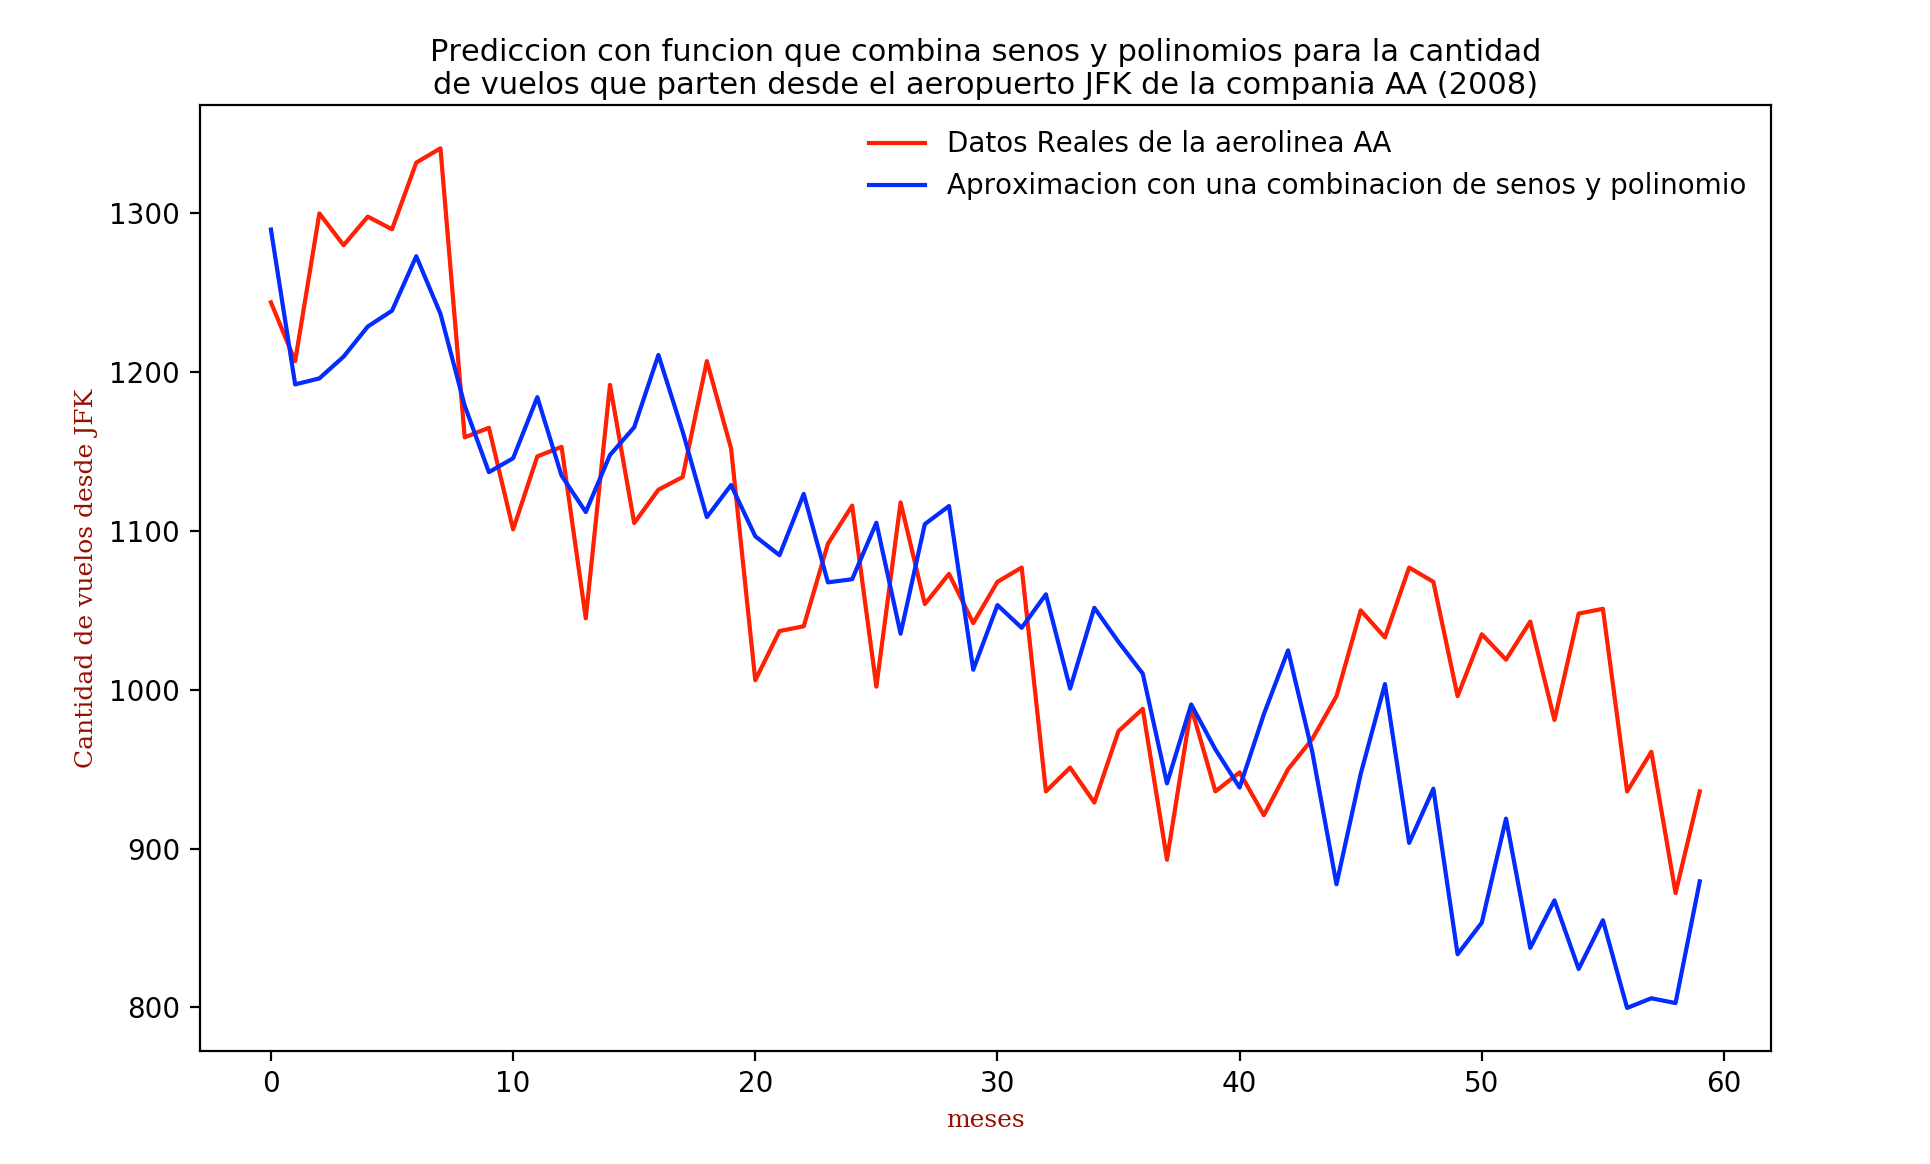
\includegraphics[scale=0.7]{imagenes/AA.png}
\end{center}

En el gr\'afico se puede observar que la funci\'on elegida se comporto de forma similar a la funcion dada por los valores reales, pero de forma mas suave. Es decir, la funci\'on propuesta no es sensible a los valores outliers que se pueden dar por picos de baja o alta demanda, por lo que en meses promedios acompa\~nara la pendiente de los datos reales, pero en mese excepcionales quedara desfazada para ir reacomodandose en el correr del tiempo.

Y para el caso de la empresa \textit{Delta} la funci\'on que hacia mejor fit sobre el set de datos fue la dada por:
x_0 * tan(mes^6)^4 + x_1 * sen(mes^8) + x_2 * sen(mes^2) + x_3 * sen(mes) +  x_4


\begin{center}
\caption{figura 1}
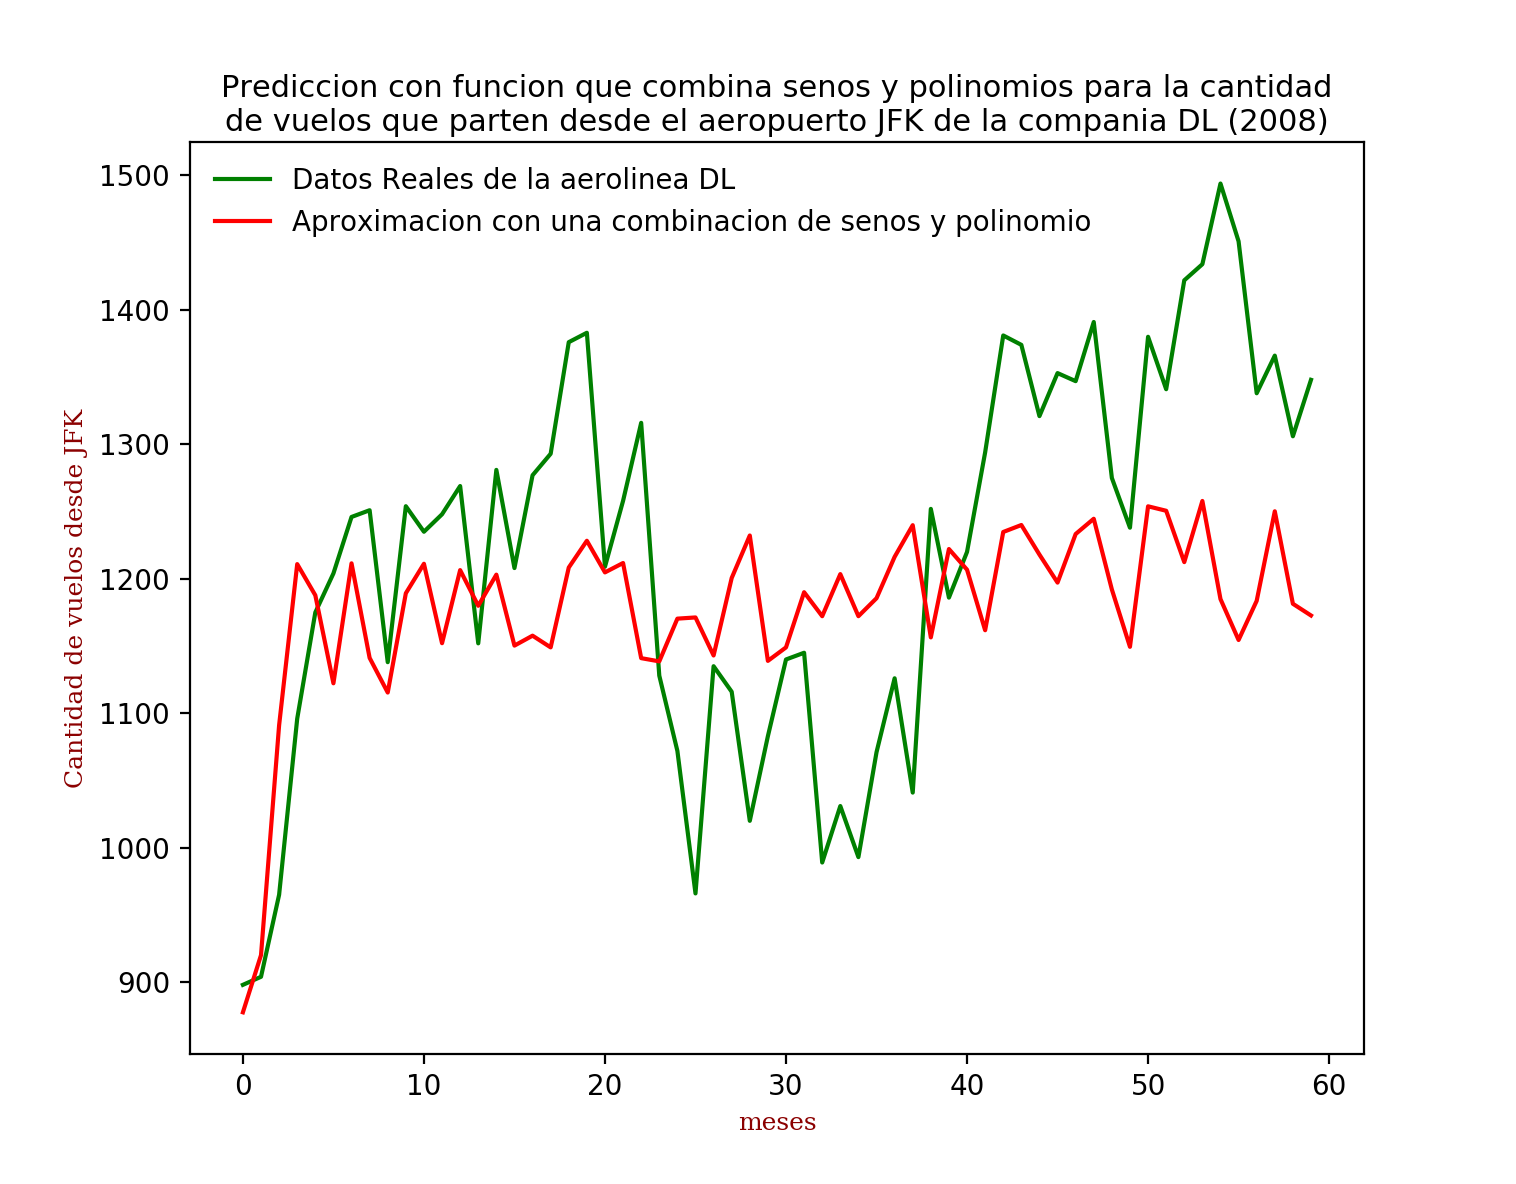
\includegraphics[scale=0.7]{imagenes/DL.png}
\end{center}

En este gr\'afico se puede observar mas el efecto de haber tomado el la funci\'on seno en varios de los coeficientes. Los saltos en la venta de pasajes son suavizados pero siguiendo la misma tendencia. Tomamos la tangente para el coeficiente asociado al x_0 porque nos permit\'ia poder representar mejor el crecimiento de de los primeros meses, sin usar una funci\'on exponencial, que en el largo plazo ser\'ia contraproducente ya que el creciemiento de ventas exponencial nunca podr\'ia ser sostenido.

